\phantomsection
\setcounter{secnumdepth}{3}

\setcounter{chapter}{1}
\chapter[{PHÂN TÍCH VÀ THIẾT KẾ HỆ THỐNG TÁC NHÂN}]{Phân tích và Thiết kế Hệ thống Tác nhân}

Chương này thiết kế các thành phần phục vụ \textbf{MT1} (CombatAgent, hàm thưởng, kiến trúc PPO), \textbf{MT2} (PCGNN + CL) và làm tiền đề cho \textbf{MT4} (biểu diễn quan sát). Để người đọc nắm được câu chuyện thiết kế thay vì chỉ thấy danh sách thành phần, chương bắt đầu bằng tổng quan quy trình huấn luyện hoàn chỉnh, sau đó ánh xạ rõ \emph{từng khối thiết kế giải quyết thách thức nào} của bài toán đã phát biểu ở chương mở đầu, sau đó đi vào chi tiết từng phần.

\section{Tổng quan quy trình huấn luyện hoàn chỉnh}
\begin{figure}[H]
    \centering
    \begin{tikzpicture}[
        >=stealth,
        node distance=0.7cm,
        box/.style={
            draw, rounded corners=3pt, 
            align=center, 
            minimum width=4.5cm, 
            minimum height=0.9cm,
            font=\small
        },
        mapbox/.style={box, fill=blue!12},
        obsbox/.style={box, fill=orange!18},
        rlbox/.style={box, fill=green!18},
        arrow/.style={->, thick}
    ]
        \node[mapbox] (pcgnn) {PCGNN sinh bản đồ};
        \node[mapbox, below=of pcgnn] (bfs) {BFS kiểm tra + phân loại dễ/khó};
        \node[mapbox, below=of bfs] (tile) {TilemapGenerator theo CL};
        \node[obsbox, below=of tile] (agent) {CombatAgent quan sát};
        \node[rlbox, below=of agent] (ppo) {PPO cập nhật chính sách};
        
        \draw[arrow] (pcgnn) -- (bfs);
        \draw[arrow] (bfs) -- (tile);
        \draw[arrow] (tile) -- (agent);
        \draw[arrow] (agent) -- (ppo);
        
        % Feedback loop (KHÔNG có label trong draw)
        \draw[arrow, dashed, blue!60] 
            (ppo.east) -- ++(1.5,0) 
            |- (tile.east);
        
        % Label đặt riêng bên PHẢI đường feedback, xoay 90 độ
        \node[font=\small\itshape, blue!60, rotate=90] 
            at ([xshift=2.0cm]$(ppo.east)!0.5!(tile.east)$) 
            {lượt chơi mới};
    \end{tikzpicture}
    \caption{Quy trình huấn luyện hoàn chỉnh. Các khối xanh là hệ thống sinh bản đồ; khối cam là quan sát; khối xanh lá là thuật toán học. Mũi tên nét đứt biểu thị vòng lặp lượt chơi.}
    \label{fig:pipeline_overview}
\end{figure}

Luồng hoạt động: PCGNN chạy ngoại tuyến để sinh tập bản đồ đa dạng; BFS lọc bản đồ hợp lệ và chia theo độ khó; TilemapGenerator nạp bản đồ đúng mức theo CL; CombatAgent thu vector quan sát từ Unity và chuyển hành động về game; PPO cập nhật chính sách dựa trên phần thưởng. Mỗi phần dưới đây đặc tả một khối trong hình này.

Bảng~\ref{tab:design_block_mapping} ánh xạ từng khối thiết kế với thách thức cụ thể của bài toán (đã phát biểu ở Chương Mở đầu) và mục tiêu MT1--MT4 mà nó phục vụ. Bảng này được dùng làm xương sống cho các section còn lại của chương.

\begin{table}[H]
    \centering
    \small
    \caption{Ánh xạ khối thiết kế $\leftrightarrow$ thách thức của bài toán $\leftrightarrow$ mục tiêu đề tài}
    \label{tab:design_block_mapping}
    \begin{tabular}{|p{3.4cm}|p{4.5cm}|p{3.5cm}|c|}
        \hline
        \textbf{Khối thiết kế} & \textbf{Thách thức giải quyết} & \textbf{Mục đặc tả} & \textbf{MT} \\
        \hline
        Quan sát 207D & Mô tả tình huống chiến đấu đủ giàu nhưng đủ gọn & §2.3 & MT1, MT4 \\
        \hline
        Hành động $(3,3,3,9)$ & Phối hợp đồng thời di chuyển--ngắm--chiến đấu & §2.4 & MT1 \\
        \hline
        Hàm thưởng định hình v1/v2 & Hướng dẫn học sớm khi tín hiệu kết quả còn thưa & §2.5 & MT1 \\
        \hline
        PCGNN + BFS & Phân phối bản đồ thay đổi mỗi lượt chơi & §2.6 & MT2 \\
        \hline
        Học theo lộ trình (CL) & Phần thưởng thưa thớt và trễ & §2.7 & MT2 \\
        \hline
        PPO + Actor-Critic & Cập nhật chính sách ổn định trên không gian hành động đa nhánh & §2.8 & MT1, MT3 \\
        \hline
    \end{tabular}
\end{table}

\section{Mô hình hóa bài toán dưới dạng POMDP}

Theo nền tảng ở Chương~1, môi trường chiến đấu được mô hình hóa như POMDP với bộ thành phần $(S, A, O, P, R, \Omega, \gamma)$, vì tác nhân không truy cập trực tiếp toàn bộ trạng thái của phòng chơi. CombatAgent chỉ nhận thông tin trong tầm nhìn VisionRadius=20 và bị ràng buộc bởi yêu cầu đường ngắm RequireLineOfSightToTarget=\textit{true}; do đó, kẻ địch hoặc đạn nằm ngoài tầm nhìn hay bị tường che khuất không xuất hiện trong quan sát. Đây là đặc tính của môi trường Roguelike chiến đấu, không phải một giới hạn tùy ý áp lên thuật toán học.


Trong bối cảnh của đề tài, mỗi thành phần POMDP tương ứng với một phần cụ thể của quá trình chơi như Bảng~\ref{tab:pomdp_mapping}. Cách ánh xạ này giúp phân biệt giữa trạng thái thật tồn tại trong Unity và quan sát hữu hạn mà chính sách thật sự nhận được.

\begin{table}[H]
    \centering
    \small
    \caption{Ánh xạ các thành phần POMDP sang môi trường Roguelike của đề tài}
    \label{tab:pomdp_mapping}
    \begin{tabular}{|p{2.7cm}|p{11.5cm}|}
        \hline
        \textbf{Thành phần} & \textbf{Ý nghĩa trong quá trình chơi} \\
        \hline
        $S$ & Trạng thái thật của phòng trong Unity: toàn bộ tilemap, vị trí/nội trạng của tác nhân, kẻ địch, đạn, hồi chiêu, va chạm, thời gian còn lại và các biến nội bộ. Trạng thái này tồn tại trong mô phỏng nhưng không được đưa nguyên vẹn cho chính sách. \\
        \hline
        $O$ & Không gian quan sát mà CombatAgent có thể nhận được sau khi Unity chuyển trạng thái thật thành vector đầu vào. Cấu hình cơ sở dùng 207 chiều; run59 dùng 210 chiều với tín hiệu dẫn đường, còn run62 dùng 432 chiều với lưới cục bộ $15\times15$. \\
        \hline
        $o_t$ & Quan sát cụ thể tại bước quyết định $t$: máu, vũ khí, hồi chiêu, vận tốc của tác nhân, các kẻ địch và viên đạn gần nhất, cùng tín hiệu tường/vật cản. Đây là lát cắt hữu hạn của trạng thái thật và là đầu vào của chính sách $\pi_\theta$. \\
        \hline
        $A$ & Không gian hành động rời rạc nhiều nhánh $(3,3,3,9)$, gồm điều khiển trục X, trục Y, lệnh chiến đấu/lướt và hướng tấn công. Cách tách nhánh giúp tác nhân phối hợp di chuyển, né tránh và ngắm bắn trong cùng một bước quyết định. \\
        \hline
        $a_t$ & Hành động cụ thể được chọn ở bước $t$, ví dụ di chuyển, lướt, giữ vị trí hoặc tấn công theo một hướng ngắm. Sau khi thực thi, Unity cập nhật vật lý, va chạm, đạn, sát thương và AI kẻ địch. \\
        \hline
        $P(s_{t+1}\mid s_t,a_t)$ & Hàm chuyển trạng thái của game: trạng thái kế tiếp phụ thuộc vào vật lý 2D, tường, đạn, sát thương, hồi chiêu, hành vi kẻ địch và logic kết thúc lượt chơi. Hàm này do Unity và TopDown Engine hiện thực, không được học trực tiếp bởi PPO. \\
        \hline
        $R(s_t,a_t)$ & Hàm phần thưởng dùng để huấn luyện: thưởng khi gây sát thương, tiêu diệt kẻ địch, dọn phòng hoặc tiếp cận mục tiêu; phạt khi nhận sát thương, đứng gần địch nhưng không hành động, bị kẹt hoặc hết thời gian. Hàm thưởng kết hợp tín hiệu kết quả thưa với định hình nhỏ. \\
        \hline
        $\Omega(o_t\mid s_t,a_{t-1})$ & Cơ chế phát quan sát từ trạng thái thật sang vector quan sát. Do tầm nhìn hữu hạn, yêu cầu đường ngắm và giới hạn số phần tử mã hóa, một số kẻ địch/đạn có thể không xuất hiện đầy đủ trong $o_t$. Đây là nguồn chính tạo tính quan sát một phần. \\
        \hline
        $\gamma$ & Hệ số chiết khấu trong PPO. Giá trị $\gamma=0.99$ giúp tác nhân không chỉ tối ưu phần thưởng tức thời mà còn học các chuỗi hành vi dài hơn như tiếp cận, né đạn, tấn công và dọn phòng. \\
        \hline
    \end{tabular}
\end{table}


Mục tiêu huấn luyện là tìm chính sách $\pi_{\theta}(a \mid o)$, tức chính sách ra quyết định dựa trên quan sát thay vì trạng thái thật, sao cho kỳ vọng tổng thưởng chiết khấu được tối đa hóa:
\begin{equation}
    J(\pi_\theta) = \mathbb{E}_{\tau \sim \pi_\theta}
    \left[\sum_{t=0}^{T}\gamma^t r_t\right].
\end{equation}

Trong công thức này, một quỹ đạo $\tau$ tương ứng với một lượt chơi hoàn chỉnh trong phòng: tác nhân được sinh ra, nhận chuỗi quan sát, chọn chuỗi hành động và kết thúc khi dọn phòng, bị hạ hoặc hết thời gian. Phần thưởng $r_t$ tại mỗi bước đến từ các tín hiệu như gây sát thương, tiêu diệt kẻ địch, dọn phòng, nhận sát thương hoặc hành vi kém hiệu quả. Vì vậy, tối đa hóa $J(\pi_\theta)$ tương ứng với việc học một chính sách vừa sống sót, vừa tiếp cận và tiêu diệt kẻ địch hiệu quả.

\textbf{Nguồn gốc tính quan sát một phần.} Trong môi trường này, tính quan sát một phần xuất hiện từ ba nguồn chính:
\begin{itemize}
    \item \textbf{Tầm nhìn hữu hạn}: game dùng Physics2D.OverlapCircle với bán kính VisionRadius=20 để truy vấn kẻ địch và đạn xung quanh tác nhân. Những đối tượng nằm ngoài bán kính này không được đưa vào tập ứng viên quan sát.
    \item \textbf{Đường ngắm bị tường chắn}: với RequireLineOfSightToTarget=\textit{true}, một kẻ địch chỉ được coi là mục tiêu hợp lệ khi giữa tác nhân và kẻ địch không có tường cản. Vì vậy, một đối tượng tuy ở gần nhưng khuất sau vật cản vẫn có thể vắng mặt khỏi quan sát hiện thời.
    \item \textbf{Dung lượng hữu hạn của vector quan sát}: do quan sát có kích thước cố định, hệ thống chỉ truyền một số lượng đối tượng giới hạn: tối đa MaxEnemies=3 kẻ địch và MaxBullets=10 viên đạn gần nhất, kèm thông tin tường dạng cục bộ (16 tia ray ở cấu hình 207 chiều, hoặc lưới $15\times15$ ở run62). Các đối tượng vượt quá giới hạn này bị cắt bỏ ngay cả khi vẫn nằm trong vùng nhận thức.
\end{itemize}

Hai nguồn đầu là thuộc tính cố hữu của luật chơi Roguelike chiến đấu: tác nhân không thể thấy xuyên tường hoặc thấy vô hạn khoảng cách. Nguồn thứ ba thuộc về lựa chọn thiết kế biểu diễn quan sát. Đây là điểm mà đề tài chủ động kiểm tra trong \textbf{MT4}, thông qua việc bổ sung tín hiệu dẫn đường BFS ở run59 và thay quan sát tường bằng lưới không gian cục bộ ở run62.

Vì $o_t$ chỉ là lát cắt hữu hạn của $s_t$, chính sách MLP dạng $\pi_\theta(a \mid o_t)$ có thể thiếu thông tin về các sự kiện vừa rời khỏi tầm nhìn, trạng thái hồi chiêu trước đó hoặc chuyển động của đạn qua nhiều bước. Về nguyên tắc, một chính sách có bộ nhớ $\pi_\theta(a \mid o_{1:t})$ có khả năng tận dụng chuỗi quan sát tốt hơn. Nhận định này dẫn đến hai hướng kiểm tra ở các chương sau: bổ sung LSTM trong run42 và run47 để khai thác lịch sử quan sát, đồng thời mở rộng không gian quan sát trong run59 và run62 để giảm mức cắt cụt thông tin.

Ngoài tính quan sát một phần, bài toán còn khó vì phân phối trạng thái thay đổi theo từng lượt chơi. Bản đồ được chọn từ nhiều bản đồ dạng văn bản khác nhau, vị trí sinh có thể cố định hoặc ngẫu nhiên theo giai đoạn CL, kẻ địch và đạn di chuyển liên tục, còn phần thưởng hoàn thành phòng chỉ xuất hiện sau khi tác nhân tiêu diệt đủ mục tiêu. Vì vậy, thiết kế $O$ phải cân bằng giữa hai yêu cầu: đủ giàu để mô tả tình huống chiến đấu tức thời, nhưng đủ gọn để PPO học hiệu quả trong ngân sách huấn luyện của đề tài.

\section{Không gian quan sát}

\textbf{Yêu cầu thiết kế.} Biểu diễn quan sát cần đủ giàu để mô tả tình huống chiến đấu (vị trí kẻ địch, đạn đang bay, tường gần), nhưng vẫn đủ gọn để PPO học được trong 1--3 triệu bước trên phần cứng đã có. Đây là phần thiết kế phục vụ trực tiếp MT1 và tạo nền cho phân tích nút thắt quan sát ở MT4.

Cách tiếp cận được chọn là tách bốn nhóm thông tin (tác nhân, kẻ địch, đạn, tường) thành các đoạn có kích thước cố định, dùng tia ray cho tường thay vì lưới chiếm chỗ để giảm chiều, và đệm bằng 0 khi số kẻ địch/đạn thay đổi giữa các lượt chơi. Nhờ đó, kích thước đầu vào luôn ổn định dù trạng thái trong phòng thay đổi theo từng lượt.

Hệ thống sử dụng quan sát dạng vector thay vì ảnh pixel. Lựa chọn này giúp giảm chi phí mẫu, tránh phải học lại các đặc trưng thị giác cơ bản, đồng thời phù hợp với mục tiêu nghiên cứu là đánh giá ảnh hưởng của CL và các kỹ thuật khám phá trên một môi trường có cấu trúc. Trong Unity Inspector, kích thước quan sát vector của behavior CombatAgentConfig được cấu hình là 207 chiều.

\begin{table}[H]
    \centering
    \small
    \caption{Cấu trúc vector quan sát 207 chiều của CombatAgent}
    \label{tab:obs_207}
    \begin{tabular}{|p{4cm}|c|p{8cm}|}
        \hline
        \textbf{Nhóm quan sát} & \textbf{Số chiều} & \textbf{Nội dung chính} \\
        \hline
        Trạng thái tác nhân & 13 & Máu, đạn, hồi chiêu, trạng thái sẵn sàng của vũ khí, tốc độ, sát thương gần đây, hướng vận tốc và giá trị đệm để giữ kích thước cố định. \\
        \hline
        Thông tin toàn cục & 4 & Tỷ lệ kẻ địch nhìn thấy, tỷ lệ đạn nhìn thấy, thời gian lượt chơi đã chuẩn hóa và giá trị đệm. \\
        \hline
        Kẻ địch gần nhất & 54 & 3 kẻ địch $\times$ 18 đặc trưng: vị trí tương đối, vận tốc tương đối, khoảng cách, máu, mức đe dọa, trạng thái tấn công, hồi chiêu và giá trị đệm. \\
        \hline
        Đạn trong vùng nhìn & 120 & 10 viên đạn $\times$ 12 đặc trưng: vị trí tương đối, vận tốc, khoảng cách, thời gian ước lượng tới va chạm, loại chủ sở hữu và giá trị đệm. \\
        \hline
        Tường/vật cản & 16 & 16 tia ray đều quanh tác nhân, mỗi tia trả về khoảng cách chuẩn hóa tới tường gần nhất. \\
        \hline
        \textbf{Tổng} & \textbf{207} & $13 + 4 + 54 + 120 + 16 = 207$. \\
        \hline
    \end{tabular}
\end{table}

% \begin{figure}[H]
% \centering
% 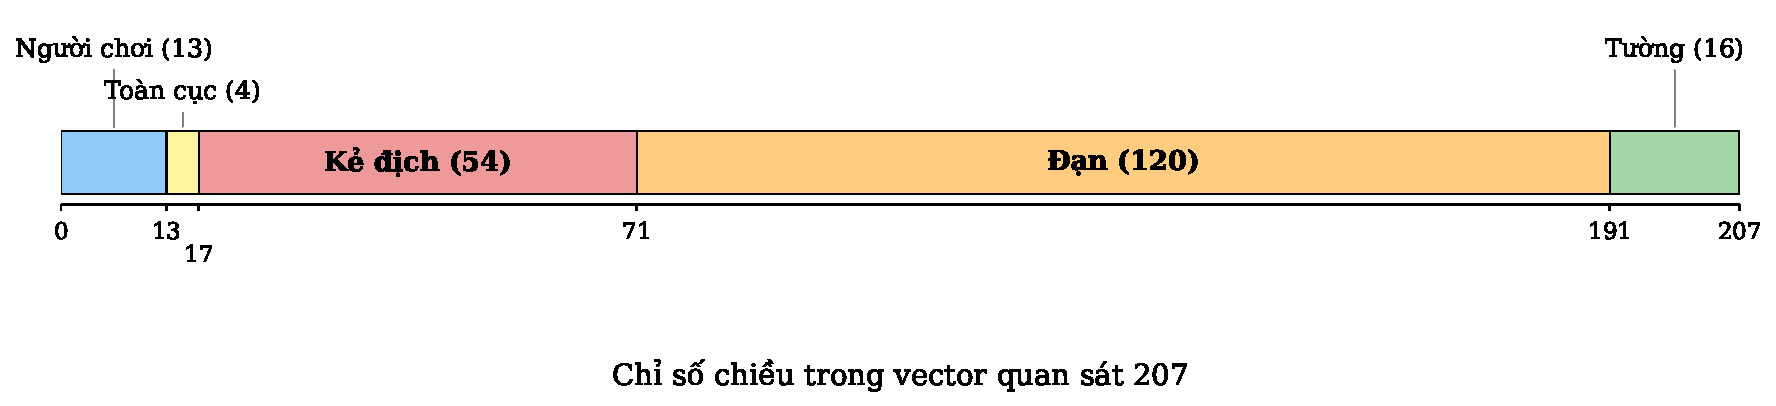
\includegraphics[width=0.95\textwidth]{figures/training/fig_obs_breakdown.pdf}
% \caption{Cấu trúc vector quan sát 207 chiều của CombatAgent, phân theo nhóm thông tin. Chiều rộng mỗi đoạn xấp xỉ tỷ lệ với số chiều; nhóm Đạn (120) chiếm hơn nửa vector, tiếp theo là Kẻ địch (54).}
% \label{fig:obs_breakdown}
% \end{figure}

Thiết kế này cố ý tách rõ thông tin tác nhân, kẻ địch, đạn và tường. Tác nhân không cần suy luận vị trí đạn từ ảnh thô, nhưng vẫn phải học cách kết hợp nhiều nguồn nguy cơ: vừa tiếp cận kẻ địch để gây sát thương, vừa tránh đạn và không mắc vào tường. Vì số lượng kẻ địch và đạn trong cảnh chơi có thể thay đổi, các nhóm đặc trưng được giới hạn bởi MaxEnemies=3 và MaxBullets=10; nếu thiếu đối tượng thì hệ thống thêm giá trị 0 để vector luôn có kích thước cố định.

\section{Không gian hành động}

Trong chiến đấu thời gian thực, tại mỗi bước tác nhân phải đồng thời quyết định: đi đâu, có tấn công/lướt hay không, và nếu tấn công thì ngắm hướng nào. Một không gian hành động một chiều (ví dụ 81 hành động phẳng) sẽ buộc PPO học từng tổ hợp như một hành động riêng, trong khi các quyết định này có phần độc lập với nhau.

Vì vậy, đề tài dùng không gian hành động rời rạc đa nhánh, tách bốn quyết định gần như độc lập thành bốn nhánh riêng. Actor sinh bốn phân phối xác suất song song; tổ hợp tổng thể là 243 hành động nhưng tham số học cho mỗi nhánh nhỏ hơn nhiều so với một softmax 243 phần tử.

CombatAgent sử dụng không gian hành động rời rạc nhiều nhánh gồm bốn nhánh với kích thước $(3,3,3,9)$. Thay vì biểu diễn toàn bộ hành vi của tác nhân bằng một tập hành động đơn lẻ, cách thiết kế này tách quyết định tại mỗi bước thời gian thành nhiều thành phần điều khiển độc lập hơn: di chuyển theo trục X, di chuyển theo trục Y, lựa chọn lệnh chiến đấu và xác định hướng tấn công. Hai nhánh đầu tiên cho phép tác nhân điều khiển hướng di chuyển trên mặt phẳng 2D, bao gồm đứng yên, di chuyển theo chiều âm hoặc chiều dương của từng trục. Nhánh thứ ba biểu diễn ý định hành động trong chiến đấu, chẳng hạn không thực hiện hành động đặc biệt, tấn công hoặc lướt. Nhánh cuối cùng xác định hướng tấn công/định hướng, giúp tác nhân căn hướng khi tương tác với kẻ địch.

Cách biểu diễn này phù hợp với đặc trưng của môi trường chiến đấu thời gian thực, nơi tác nhân không chỉ cần chọn một hành vi tổng quát tại mỗi thời điểm mà còn phải phối hợp đồng thời nhiều quyết định nhỏ. Ví dụ, tác nhân có thể vừa di chuyển để né đạn, vừa giữ khoảng cách với kẻ địch, đồng thời lựa chọn thời điểm tấn công và hướng tấn công phù hợp. Do đó, một hành động của CombatAgent không phải là một lệnh đơn lẻ, mà là tổ hợp của nhiều quyết định điều khiển diễn ra trong cùng một bước thời gian. Thiết kế này giúp mô hình hóa tự nhiên hơn các hành vi chiến đấu như tiếp cận, né tránh, lướt khỏi vùng nguy hiểm, căn hướng và tấn công trong môi trường Roguelike.

\begin{table}[H]
    \centering
    \small
    \caption{Không gian hành động rời rạc nhiều nhánh của CombatAgent}
    \label{tab:action_space}
    \begin{tabular}{|c|c|p{9cm}|}
        \hline
        \textbf{Nhánh} & \textbf{Kích thước} & \textbf{Ý nghĩa} \\
        \hline
        0 & 3 & moveX: không di chuyển theo trục X, sang trái, sang phải. \\
        \hline
        1 & 3 & moveY: không di chuyển theo trục Y, đi xuống, đi lên. \\
        \hline
        2 & 3 & chiến đấu: không hành động, tấn công, lướt. Các lựa chọn tấn công hoặc lướt được lọc khỏi tập hành động hợp lệ khi vũ khí/kỹ năng chưa sẵn sàng. \\
        \hline
        3 & 9 & aim: giữ hướng cũ hoặc ngắm theo 8 hướng rời rạc. \\
        \hline
    \end{tabular}
\end{table}

\begin{figure}[H]
\centering
\begin{tikzpicture}[
  every node/.style={font=\small},
  rootnode/.style={draw, rounded corners=4pt, fill=orange!25, minimum width=4.0cm, minimum height=0.85cm, align=center},
  branchnode/.style={draw, rounded corners=3pt, minimum width=2.4cm, minimum height=0.85cm, align=center},
  leafbox/.style={draw=gray!55, rounded corners=2pt, minimum width=2.4cm, minimum height=1.55cm, align=center, font=\scriptsize, fill=gray!8},
  totalbox/.style={draw, rounded corners=3pt, fill=yellow!18, minimum width=8.5cm, minimum height=0.7cm, align=center, font=\small},
  >=stealth
]
% Root
\node[rootnode] (root) at (0,0) {Hành động $a_t$\\(multi-discrete, 4 nhánh độc lập)};

% 4 branches
\node[branchnode, fill=blue!15]  (mX) at (-6.0,-1.7) {moveX\\(3)};
\node[branchnode, fill=cyan!18]  (mY) at (-2.0,-1.7) {moveY\\(3)};
\node[branchnode, fill=red!15]   (cb) at ( 2.0,-1.7) {combat\\(3)};
\node[branchnode, fill=green!18] (am) at ( 6.0,-1.7) {aim\\(9)};

\draw[->] (root.south) -- (mX.north);
\draw[->] (root.south) -- (mY.north);
\draw[->] (root.south) -- (cb.north);
\draw[->] (root.south) -- (am.north);

% Leaves
\node[leafbox] (lX) at (-6.0,-3.6) {không\\trái\\phải};
\node[leafbox] (lY) at (-2.0,-3.6) {không\\xuống\\lên};
\node[leafbox] (lC) at ( 2.0,-3.6) {không\\tấn công\\lướt};
\node[leafbox] (lA) at ( 6.0,-3.6) {giữ + 8 hướng};

\draw[->, gray!70] (mX) -- (lX);
\draw[->, gray!70] (mY) -- (lY);
\draw[->, gray!70] (cb) -- (lC);
\draw[->, gray!70] (am) -- (lA);

% Total annotation
\node[totalbox] at (0,-5.0)
  {Tổng tổ hợp: $3 \times 3 \times 3 \times 9 = 243$\quad(81 tổ hợp \emph{di chuyển $\times$ ngắm} nếu bỏ qua combat)};
\end{tikzpicture}
\caption{Cấu trúc cây của không gian hành động $(3,3,3,9)$ của CombatAgent. Bốn nhánh được chọn độc lập tại mỗi bước, tạo 243 tổ hợp tổng cộng trước khi cơ chế lọc hành động hợp lệ loại bỏ các hành động không hợp lệ. Riêng tổ hợp di chuyển (9 hướng) $\times$ ngắm (9 hướng) đã đạt 81 trạng thái điều khiển.}
\label{fig:action_space_tree}
\end{figure}

Tổ hợp hai nhánh moveX và moveY tạo ra 9 hướng di chuyển (bao gồm đứng yên), trong khi nhánh aim điều khiển hướng tấn công. Entropy cực đại lý thuyết của không gian hành động, nếu mọi lựa chọn đều hợp lệ và phân phối đều, là:

\begin{equation}
    H_{\max} = \ln(3) + \ln(3) + \ln(3) + \ln(9) \approx 5.49 \text{ nat}.
    \label{eq:max_entropy}
\end{equation}

Giá trị này được dùng lại trong Chương~4 khi phân tích hiện tượng bão hòa entropy. Lưu ý là cơ chế lọc hành động hợp lệ có thể làm entropy cực đại thực tế thấp hơn tại một số trạng thái, vì các hành động như tấn công hoặc lướt không phải lúc nào cũng hợp lệ.

\section{Thiết kế hàm phần thưởng}

Tín hiệu kết quả thật (hạ kẻ địch, dọn phòng) xuất hiện quá thưa để PPO khám phá hiệu quả trong giai đoạn đầu. Ngược lại, nếu phần thưởng định hình quá lớn, tác nhân có thể tối ưu hành vi trung gian như chỉ tiếp cận kẻ địch mà không thực sự tấn công.

Hàm thưởng vì vậy kết hợp hai nhóm tín hiệu. Nhóm kết quả giữ giá trị tuyệt đối lớn để phản ánh mục tiêu thật; nhóm định hình giữ giá trị nhỏ và được giảm thêm ở phiên bản v2 để tránh chi phối hành vi cuối. Phiên bản v2 cũng tăng trọng số cho kết quả và phạt mạnh hơn hành vi chần chừ, nhằm kiểm tra liệu tác nhân có trở nên quyết đoán hơn hay không (đánh giá ở Chương~4).

Hàm thưởng kết hợp phần thưởng kết quả thưa và phần thưởng định hình dày. Nhóm phần thưởng kết quả thưa phản ánh mục tiêu thật của phòng chơi, còn phần thưởng định hình cung cấp tín hiệu học trung gian để PPO không bị kẹt trong giai đoạn chưa từng hoàn thành phòng.

\begin{table}[H]
    \centering
    \small
    \caption{Các thành phần thưởng chính trong hai phiên bản hàm thưởng}
    \label{tab:reward_components}
    \begin{tabular}{|p{4.4cm}|c|c|p{5.2cm}|}
        \hline
        \textbf{Sự kiện} & \textbf{v1} & \textbf{v2} & \textbf{Vai trò} \\
        \hline
        Gây sát thương & $+1.0$ & $+1.5$ & Khuyến khích gây sát thương thay vì chỉ né tránh. \\
        \hline
        Hạ một kẻ địch & $+3.0$ & $+5.0$ & Tín hiệu kết quả thưa nhưng có ý nghĩa chiến thuật cao. \\
        \hline
        Dọn sạch toàn bộ phòng & $+5.0$ & $+10.0$ & Mục tiêu cuối của lượt chơi; hàm thưởng v2 tăng mạnh tín hiệu hoàn thành. \\
        \hline
        Tiếp cận mục tiêu & $+0.008 \times \Delta d$ & $+0.003 \times \Delta d$ & Định hình theo khoảng cách, giảm ở v2 để tránh tác nhân chỉ tối ưu hành vi tiếp cận. \\
        \hline
        Tấn công đúng hướng & $+0.05$ & $+0.15$ & Tăng phần thưởng cho ý định tấn công có căn chỉnh tốt. \\
        \hline
        Đứng gần địch không hành động & $-0.0005$ & $-0.002$ & Phạt hành vi chần chừ trong vùng nguy hiểm. \\
        \hline
        Tác nhân chết & $-2.0$ & $-2.0$ & Tín hiệu kết thúc âm. \\
        \hline
    \end{tabular}
\end{table}

Bảng~\ref{tab:reward_components} chỉ liệt kê các thành phần chính. Trong hiện thực, mã nguồn còn có các tín hiệu nhỏ hơn như phạt theo thời gian, phạt nhận sát thương, thưởng lướt hữu ích, phạt tấn công không hợp lệ và phần thưởng căn chỉnh hướng tấn công. Cấu hình v1 được dùng cho các lần chạy chính từ run34 đến run54. Cấu hình v2 được dùng trong run55 như một thí nghiệm thay đổi thang thưởng, vì vậy các giá trị phần thưởng trung bình của run55 không được so trực tiếp với các lần chạy v1.

\section{Sinh bản đồ bằng PCGNN và TilemapGenerator}

Để giải quyết thách thức bản đồ thay đổi qua từng lượt chơi (MT2), tác nhân cần được huấn luyện trên nhiều bản đồ thay vì một bố cục cố định. Tuy nhiên, gọi trực tiếp generator Python từ Unity ở mỗi lượt chơi tạo độ trễ và rủi ro lỗi tích hợp; mặt khác sinh bản đồ không kiểm tra có thể tạo ra bố cục nơi tác nhân và kẻ địch nằm trên hai vùng tách rời.

Vì vậy, hệ thống được tách thành hai tầng: PCGNN chạy ngoại tuyến để sinh và kiểm tra hợp lệ, còn TilemapGenerator trong Unity chỉ đọc các bản đồ đã tuyển chọn. Cách này vừa giữ tính đa dạng vừa giảm rủi ro tích hợp lúc chạy.

Môi trường huấn luyện dùng quy trình hai tầng. Tầng thứ nhất là PCGNN chạy ngoại tuyến ở phía Python để sinh nhiều bản đồ từ một genome đã huấn luyện. Tầng thứ hai là TilemapGenerator trong Unity, có nhiệm vụ đọc các bản đồ dạng văn bản đã được tuyển chọn, chuyển thành tilemap, chọn vị trí sinh và đưa phòng vào lượt chơi huấn luyện. Thiết kế này giữ được tính đa dạng của PCGNN nhưng tránh việc gọi Python trực tiếp trong mỗi lượt chơi Unity, nhờ đó giảm rủi ro độ trễ và lỗi tích hợp trong quá trình huấn luyện.

NEAT tiến hóa quần thể genome qua nhiều thế hệ; mỗi genome mã hóa một mạng sinh tile. Fitness kết hợp tỷ lệ bản đồ hợp lệ, novelty nội bộ, novelty so với archive và độ phủ MAP-Elites. MAP-Elites chia không gian đặc trưng bản đồ (wall\_ratio, path\_length) thành các ô và lưu generator tốt nhất mỗi ô, ngăn quần thể hội tụ về một kiểu bản đồ duy nhất. Chi tiết cơ chế NEAT và novelty search trong \cite{Beukman2022}.


Mỗi bản đồ sau khi sinh được chuẩn hóa về định dạng văn bản của trò chơi: ký tự \# biểu diễn tường, . biểu diễn sàn, P là vị trí sinh tác nhân và E là vị trí sinh kẻ địch. Vì đầu ra của PCGNN chủ yếu là ma trận tile, đề tài bổ sung một bộ chuyển đổi để đặt P/E trên cùng một thành phần liên thông của vùng sàn. Sau đó hệ thống chạy BFS để kiểm tra tác nhân có thể đi tới kẻ địch hay không trước khi bản đồ được đưa vào tập huấn luyện.

\begin{figure}[H]
    \centering
    \begin{tikzpicture}[node distance=1.7cm, >=stealth, every node/.style={font=\small}]
        \node[draw, rounded corners, align=center, minimum width=2.7cm, minimum height=0.9cm] (pcgnn) {PCGNN\\genome};
        \node[draw, rounded corners, align=center, right of=pcgnn, xshift=2.0cm, minimum width=2.9cm, minimum height=0.9cm] (adapter) {Bộ chuyển đổi\\dạng văn bản};
        \node[draw, rounded corners, align=center, right of=adapter, xshift=2.0cm, minimum width=3.0cm, minimum height=0.9cm] (metric) {BFS + chỉ số\\độ khó};
        \node[draw, rounded corners, align=center, below of=adapter, yshift=-0.4cm, minimum width=3.2cm, minimum height=0.9cm] (tiers) {Dễ/Trung bình/Khó\\thư mục};
        \node[draw, rounded corners, align=center, right of=tiers, xshift=2.0cm, minimum width=3.0cm, minimum height=0.9cm] (unity) {TilemapGenerator\\lượt chơi Unity};
        \draw[->] (pcgnn) -- (adapter);
        \draw[->] (adapter) -- (metric);
        \draw[->] (metric) -- (tiers);
        \draw[->] (tiers) -- (unity);
    \end{tikzpicture}
    \caption{Luồng sinh và tuyển chọn bản đồ bằng PCGNN trước khi đưa vào Unity}
    \label{fig:map_generation_workflow}
\end{figure}

\begin{figure}[H]
    \centering
    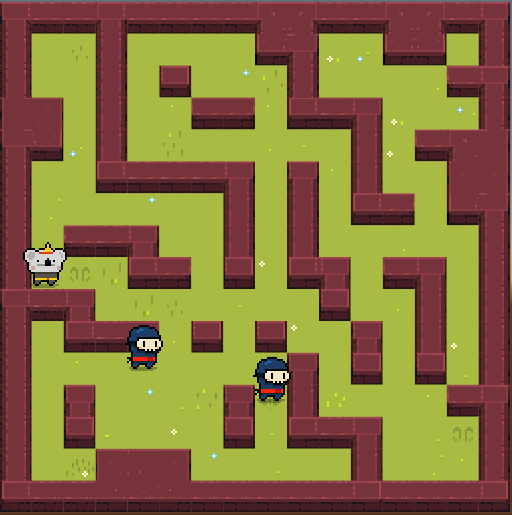
\includegraphics[width=0.72\textwidth]{figures/map_gen.png}
    \caption{Ví dụ bản đồ sau khi được dựng trong môi trường Unity từ bản đồ dạng văn bản}
    \label{fig:unity_generated_map_example}
\end{figure}

Độ khó bản đồ được đánh giá bằng các chỉ số hình học gồm tỷ lệ tường, độ dài đường đi ngắn nhất giữa P và E, tỷ lệ ngõ cụt, tỷ lệ vùng có thể đi tới và độ khó A*. Trong phiên bản sử dụng cho tập bản đồ hiện tại, điểm độ khó được tính theo công thức:

\begin{equation}
\begin{aligned}
    \text{difficulty\_score} ={} & 0.90 \times \text{wall\_ratio} + 0.05 \times \min(\text{path\_norm}, 1.0) \\
    & {}+ 0.03 \times \text{dead\_end\_ratio} + 0.02 \times \text{astar\_difficulty}.
\end{aligned}
\label{eq:map_difficulty_score}
\end{equation}

Trong công thức~\ref{eq:map_difficulty_score}, \emph{wall\_ratio} được gán trọng số cao nhất vì mật độ tường ảnh hưởng trực tiếp đến không gian di chuyển và mức độ phức tạp của bản đồ. Do đó, \emph{difficulty\_score} trong khóa luận chủ yếu là chỉ số sắp xếp độ phức tạp hình học, không phải thước đo đầy đủ cho mọi khía cạnh độ khó chiến đấu. Các thành phần còn lại như độ dài đường đi, tỷ lệ ngõ cụt và độ khó A* đóng vai trò bổ trợ, giúp tinh chỉnh thứ hạng độ khó thay vì chi phối hoàn toàn kết quả phân loại. Thay vì đặt ngưỡng tuyệt đối cứng cho mọi generator, hệ thống có thể sắp xếp bản đồ theo độ khó tương đối: 5\% dễ nhất được đưa vào Dễ, 5\% tiếp theo vào Trung bình và phần còn lại vào Khó. Cách chia này phù hợp với giai đoạn tuyển chọn thủ công vì người thiết kế vẫn có thể xem lại từng thư mục và chọn những bản đồ tốt nhất trước khi đưa sang Unity.

\textbf{Tập bản đồ đưa vào Unity.} Ở giai đoạn sinh bản đồ ban đầu, tập bản đồ PCGNN chính có 1000 bản đồ kích thước $14\times14$ và được chia theo tỷ lệ 5/5/90 để tạo ba nhóm Dễ, Trung bình và Khó. Tuy nhiên, khóa luận không sử dụng toàn bộ 1000 bản đồ này trong Unity. Thay vào đó, các bản đồ được xem xét thủ công theo tính hợp lệ, khả năng đi tới và chất lượng bố cục, sau đó chỉ một tập con đại diện được gán trực tiếp cho các thí nghiệm hiện tại, gồm 5 bản đồ Dễ, 5 bản đồ Trung bình và 50 bản đồ Khó. Cách dùng tập con này giúp kiểm soát chất lượng bản đồ trước khi mở rộng phân loại đầy đủ: hai nhóm Dễ và Trung bình đóng vai trò tạo tín hiệu học ban đầu trong giai đoạn đầu, còn nhóm Khó là phân phối mục tiêu chiếm phần lớn thời gian huấn luyện.

\begin{table}[H]
    \centering
    \small
    \caption{Phân bố bản đồ đang gán trong Unity theo nhóm độ khó}
    \label{tab:map_split}
    \begin{tabular}{|p{2.5cm}|c|c|p{7.5cm}|}
        \hline
        \textbf{Nhóm} & \textbf{Số bản đồ} & \textbf{Tỷ lệ} & \textbf{Vai trò trong huấn luyện} \\
        \hline
        Dễ   & 5  & 8.33\%  & Tạo tín hiệu học ban đầu cho giai đoạn $\sim$0--70k bước; tập nhỏ đã được chọn để tác nhân có cơ hội hoàn thành phòng thường xuyên hơn. \\
        \hline
        Trung bình & 5  & 8.33\%  & Bước trung gian từ Dễ sang Khó, dùng khoảng $\sim$70k--140k bước. \\
        \hline
        Khó   & 50 & 83.33\% & Phân phối mục tiêu, chiếm hơn 95\% thời gian huấn luyện; số lượng lớn hơn hai nhóm đầu để tăng đa dạng bố cục. \\
        \hline
    \end{tabular}
\end{table}

Trong Unity, TilemapGenerator không cần biết bản đồ được vẽ tay hay sinh bằng PCGNN. Thành phần này chỉ đọc \texttt{TextAsset} của Unity theo nhóm hiện tại, dựng tilemap và kiểm tra lại vùng có thể đi tới. Với các giai đoạn dùng vị trí sinh cố định, TilemapGenerator ưu tiên ô sàn có độ phủ BFS tốt để tránh trường hợp tác nhân hoặc kẻ địch bị cô lập. Với các giai đoạn dùng vị trí sinh ngẫu nhiên, tác nhân và kẻ địch được chọn từ các ô sàn hợp lệ nhằm tăng phương sai môi trường. Hình~\ref{fig:unity_tilemap_generator_inspector} minh họa cấu hình TilemapGenerator trong Inspector, trong đó Unity đang dùng chế độ CL với 5 bản đồ Dễ, 5 bản đồ Trung bình và 50 bản đồ Khó.

\begin{figure}[H]
    \centering
    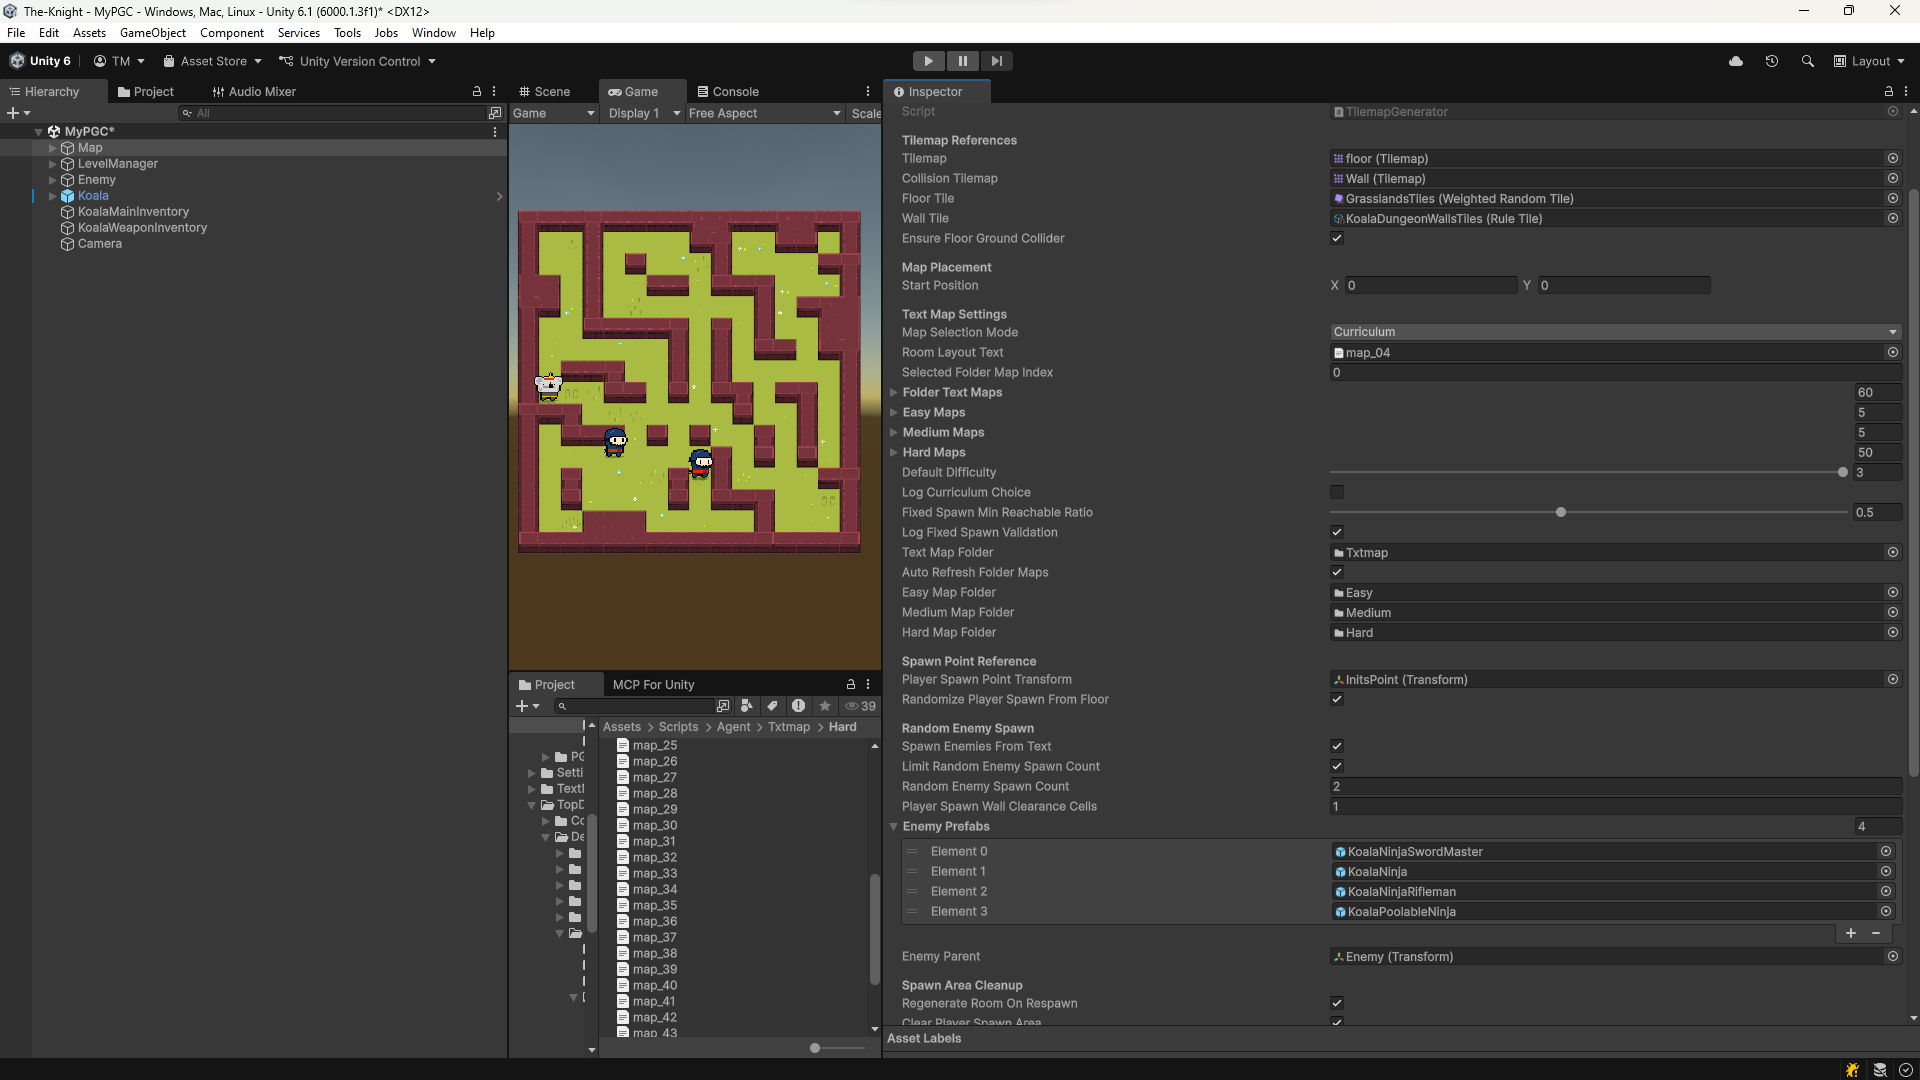
\includegraphics[width=0.98\textwidth]{figures/unity_env.png}
    \caption{Cấu hình TilemapGenerator trong Unity Inspector và ví dụ bản đồ đang được dựng trong Game view}
    \label{fig:unity_tilemap_generator_inspector}
\end{figure}

Bảng~\ref{tab:difficulty_spawn_policy} tóm tắt cách chọn bản đồ và vị trí sinh theo từng mức độ khó. Trong các lần chạy dùng CL, tham số môi trường \emph{difficulty} do ML-Agents truyền vào quyết định cả thư mục bản đồ và chế độ sinh. Với \emph{difficulty}=0, 1 và 2, hệ thống dùng vị trí sinh cố định: tác nhân được đặt theo quy tắc xác định trên mỗi bản đồ, còn kẻ địch được chọn từ các ô sàn có thể đi tới, trải theo nhiều mức khoảng cách để tránh xuất hiện quá gần hoặc quá xa. Với \emph{difficulty}=3, hệ thống vẫn dùng tập Khó nhưng chuyển sang sinh ngẫu nhiên sau mỗi lượt chơi. Trong cấu hình chính, mỗi lượt chơi sinh tối đa \emph{randomEnemySpawnCount}=2 kẻ địch; nếu có nhiều prefab, loại kẻ địch được lấy từ mảng \emph{enemyPrefabs}.

\begin{table}[H]
    \centering
    \small
    \caption{Chính sách chọn bản đồ và vị trí sinh theo tham số \emph{difficulty}}
    \label{tab:difficulty_spawn_policy}
    \makebox[\textwidth][c]{%
    \begin{tabular}{|c|p{2.3cm}|p{2.5cm}|p{4.0cm}|p{4.0cm}|}
        \hline
        \textbf{\emph{difficulty}} & \textbf{Nhóm bản đồ} & \textbf{Chế độ sinh} & \textbf{Vị trí sinh tác nhân} & \textbf{Vị trí sinh kẻ địch} \\
        \hline
        0 & Dễ & Cố định & Một ô sàn hợp lệ được chọn xác định cho từng bản đồ, ưu tiên vùng có không gian di chuyển tốt. & Tối đa 2 kẻ địch ở các ô sàn hợp lệ, có thể đi tới từ tác nhân và phân bố ở khoảng cách trung bình. \\
        \hline
        1 & Trung bình & Cố định & Giữ quy tắc sinh cố định như mức Dễ nhưng dùng tập bản đồ phức tạp hơn. & Giữ quy tắc sinh kẻ địch cố định để giảm phương sai khi tác nhân học bản đồ khó hơn. \\
        \hline
        2 & Khó & Cố định & Dùng tập Khó nhưng vẫn cố định vị trí sinh theo từng bản đồ. & Kẻ địch vẫn được đặt xác định theo bản đồ để tác nhân học kỹ năng chiến đấu trên cấu trúc khó trước. \\
        \hline
        3 & Khó & Ngẫu nhiên & Chọn ngẫu nhiên một ô sàn hợp lệ ở mỗi lượt chơi. & Chọn ngẫu nhiên tối đa 2 ô sàn hợp lệ có thể đi tới từ tác nhân, nhằm tăng khả năng khái quát hóa với vị trí sinh mới. \\
        \hline
    \end{tabular}
    }
\end{table}

Như vậy, độ khó không chỉ tăng vì bản đồ chuyển từ Dễ sang Trung bình và Khó, mà còn vì phương sai vị trí sinh được mở rộng ở giai đoạn Khó ngẫu nhiên. Cách tách này giúp tác nhân học trước các kỹ năng cơ bản như tiếp cận, né đạn và căn hướng tấn công trong môi trường ít nhiễu hơn, rồi mới phải thích nghi với vị trí sinh thay đổi mạnh.

\section{Khung học theo lộ trình}

Khi tác nhân khởi tạo ngẫu nhiên và phải học ngay trên nhóm Khó, phần thưởng xuất hiện rất thưa; xác suất tình cờ dọn được phòng gần như bằng 0, nên PPO không có tín hiệu học hiệu quả. Để phục vụ MT2, hệ thống cần một cơ chế tạo tín hiệu học sớm mà không phải sửa thuật toán PPO.

Học theo lộ trình tổ chức bài toán thành chuỗi từ dễ đến khó: bắt đầu ở mức Dễ (mật độ tường thấp, không gian rộng) nơi tác nhân thường xuyên hoàn thành phòng, dùng EMA của phần thưởng làm điều kiện chuyển sang Trung bình rồi Khó. ML-Agents cung cấp cơ chế truyền tham số \emph{difficulty} từ trainer xuống môi trường, gắn trực tiếp với TilemapGenerator.

CL được dùng để giảm độ khó khám phá ban đầu \cite{Bengio2009}. Thay vì đưa tác nhân ngay vào toàn bộ nhóm Khó, hệ thống bắt đầu từ bản đồ dễ hơn, chuyển sang Trung bình khi phần thưởng làm mượt vượt ngưỡng, rồi mới chuyển sang nhóm bản đồ Khó. Tham số độ khó được truyền qua Academy.Instance.EnvironmentParameters với tên difficulty.

\begin{figure}[H]
    \centering
    \begin{tikzpicture}[>=stealth,
        level/.style={draw, rounded corners, align=center, minimum width=3.0cm, minimum height=0.9cm, font=\small},
        transition/.style={font=\scriptsize, fill=white, inner sep=1.5pt}]
        \node[level] (easy) at (0,0) {Mức 0\\Dễ};
        \node[level] (medium) at (5.0,0) {Mức 1\\Trung bình};
        \node[level] (hard) at (10.0,0) {Mức 2\\Khó};
        \node[level, minimum width=3.2cm] (random) at (10.0,-1.8) {Mức 3\\Khó ngẫu nhiên};
        \draw[->] (easy.east) -- node[transition, above]{thưởng $\geq T_0$} (medium.west);
        \draw[->] (medium.east) -- node[transition, above]{thưởng $\geq T_1$} (hard.west);
        \draw[->, dashed] (hard.south) -- node[transition, right]{thưởng $\geq T_2$} (random.north);
    \end{tikzpicture}
    \caption{Cấu trúc CL 3 bậc và biến thể 4 bậc chuyển từ vị trí sinh cố định sang ngẫu nhiên}
    \label{fig:curriculum_structure}
\end{figure}

Trong run46, CL gồm 3 mức độ khó: Dễ, Trung bình và Khó. Trong run54, CL được mở rộng thành 4 mức: \emph{Dễ cố định}, \emph{Trung bình cố định}, \emph{Khó cố định} và \emph{Khó ngẫu nhiên}. Biến thể 4 bậc kiểm tra giả thuyết rằng việc giảm phương sai vị trí sinh ở giai đoạn đầu có thể giúp PPO ổn định hơn trước khi chuyển sang phân phối khó hơn.

Cần phân biệt hai lớp tổ chức độ khó. Lớp thứ nhất là chia tập bản đồ PCGNN thành các thư mục Dễ, Trung bình và Khó dựa trên chỉ số hình học. Lớp thứ hai là cơ chế chuyển mức độ khó trong ML-Agents: trainer thay đổi tham số \emph{difficulty} khi phần thưởng làm mượt vượt ngưỡng, từ đó TilemapGenerator chọn thư mục bản đồ và chế độ sinh tương ứng.

\section{Kiến trúc mạng và cấu hình PPO}

Để phục vụ MT1 và MT3, kiến trúc mạng và các siêu tham số PPO cần đủ ổn định để các lần chạy thí nghiệm cô lập biến chỉ khác nhau ở \emph{đúng một biến} (CL, ICM, RND, LSTM\dots). Nếu không, chênh lệch kết quả có thể bị quy nhầm cho kỹ thuật được kiểm tra trong khi nguyên nhân thực sự nằm ở siêu tham số.

Cấu hình cơ sở vì vậy cố định MLP actor-critic hai lớp 256 đơn vị (hidden\_units=256, num\_layers=2) và giữ nguyên các siêu tham số PPO chính giữa các lần chạy thí nghiệm cô lập biến; chỉ thay đổi biến cần kiểm tra. Các lần chạy LSTM bổ sung bộ nhớ nhưng giữ phần MLP nền.

Chính sách được huấn luyện bằng PPO trong Unity ML-Agents \cite{Juliani2018}. Cấu hình nền dùng mạng MLP actor-critic với hidden\_units=256, num\_layers=2, normalize=true. Actor head sinh phân phối xác suất cho bốn nhánh hành động, còn critic head ước lượng $V(s)$ để tính lợi thế theo GAE.

\begin{figure}[H]
    \centering
    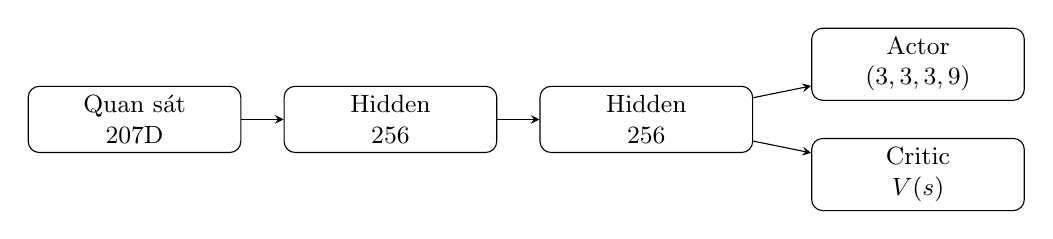
\begin{tikzpicture}[node distance=1.45cm, >=stealth, every node/.style={font=\small}]
        \node[draw, rounded corners, align=center, minimum width=2.7cm] (obs) {Quan sát\\207D};
        \node[draw, rounded corners, align=center, right of=obs, xshift=1.8cm, minimum width=2.7cm] (h1) {Hidden\\256};
        \node[draw, rounded corners, align=center, right of=h1, xshift=1.8cm, minimum width=2.7cm] (h2) {Hidden\\256};
        \node[draw, rounded corners, align=center, right of=h2, xshift=2.0cm, yshift=0.7cm, minimum width=2.7cm] (actor) {Actor\\$(3,3,3,9)$};
        \node[draw, rounded corners, align=center, right of=h2, xshift=2.0cm, yshift=-0.7cm, minimum width=2.7cm] (critic) {Critic\\$V(s)$};
        \draw[->] (obs) -- (h1);
        \draw[->] (h1) -- (h2);
        \draw[->] (h2) -- (actor);
        \draw[->] (h2) -- (critic);
    \end{tikzpicture}
    \caption{Kiến trúc actor-critic dùng cho CombatAgentConfig}
    \label{fig:actor_critic_architecture}
\end{figure}

Một số lần chạy thí nghiệm cô lập biến bổ sung bộ nhớ LSTM với memory\_size=256 và sequence\_length=64 để kiểm tra giả thuyết rằng thông tin lịch sử có thể giúp tác nhân xử lý đạn, hồi chiêu và tình huống khuất tầm nhìn. Kết quả định lượng của các lựa chọn kiến trúc này được trình bày ở Chương~4.

Chính sách dùng MLP actor-critic (hidden\_units=256, num\_layers=2, normalize=true). Actor sinh phân phối xác suất cho 4 nhánh hành động; Critic ước lượng $V(s)$ làm mốc nền cho GAE. Các lần chạy LSTM bổ sung memory\_size=256, sequence\_length=64. Các siêu tham số PPO chính (learning\_rate=$3\times10^{-4}$, batch\_size=1024, buffer\_size=10240, num\_epoch=3, $\gamma$=0.99, $\lambda$=0.95, $\epsilon$=0.2, $\beta$=$5\times10^{-3}$) được giữ thống nhất giữa các lần chạy thí nghiệm cô lập biến run34--run54 để cô lập tác động của từng kỹ thuật. Chi tiết các thay đổi trong run62 được trình bày ở Chương~3.
